%%%%%%%%%%%%%%%%%%%%%%%%%%%%%%%%%%%%%%%%%%%%%%%%%%%%%%%%%%%%%%%%%%%%%%%%%%%%%%%
% Chapter 3: Resultados
%%%%%%%%%%%%%%%%%%%%%%%%%%%%%%%%%%%%%%%%%%%%%%%%%%%%%%%%%%%%%%%%%%%%%%%%%%%%%%%

%++++++++++++++++++++++++++++++++++++++++++++++++++++++++++++++++++++++++++++++
Este capítulo se centrará en explicar las características que incorpora {\it ghedsh} tras la etapa de desarrollo tratada en el capítulo anterior.
\bigskip

Se hará una distinción entre comandos del núcleo y comandos incorporados ({\it built-in commands}). Los comandos del núcleo, son aquellos que no trabajan con los datos de GitHub del usuario pero que, sin embargo, son
esenciales desde el punto de vista de la usabilidad y experiencia de usuario con el CLI.
\bigskip

Además, los comandos incorporados sí trabajan con los datos de GitHub del usuario identificado. Permiten realizar diversas tareas, priorizando la rapidez en la ejecución de las mismas y la facilidad de uso de la herramienta.

%---------------------------------------------------------------------------------
\section{Autenticación con credenciales de GitHub}
\label{3:sec:1}

El contenido de esta sección pretende explicar el proceso de autenticación que debe seguir el usuario al usar {\it ghedsh} por primera vez.
\bigskip

Dicho proceso es necesario, puesto que se trabajan con los datos que dispone el usuario en GitHub. Además, la API REST v3 requiere, para ciertas consultas (en especial, modificaciones como crear repositorios, equipos y administrar la configuración), verificar la identidad del usuario. Si no fuera así, se podrían llevar a cabo comportamientos indeseados.
\bigskip

En {\it ghedsh}, se realiza la autenticación con {\it OAuth access token}\cite{B16}, que consiste, en una definición muy simplificada, en una cadena de caracteres alfanuméricos que actúa como una contraseña. No obstante,
en este caso de uso es mucho más potente y segura. Las principales ventajas son:
\begin{itemize}
	\item Es revocable, es decir, el {\it token} puede dejar de ser válido, eliminando el acceso para ese {\it token} en particular, sin que el usuario tenga que cambiar su contraseña en todos sus accesos.
	\item Sus permisos son configurables, esto es, un {\it token} puede ser válido sólo para ciertos recursos de una API. De esta manera, se conceden permisos de forma más controlada.
\end{itemize}

Para sintetizar este apartado, el usuario que utilice por primera vez {\it ghedsh}, debe verificar su identidad mediante sus credenciales (nombre de usuario y contraseña) de GitHub y se
generará de forma automática un {\it token} de acceso con los permisos necesarios para usar la herramienta.

\begin{figure}[H]
	\begin{center}
	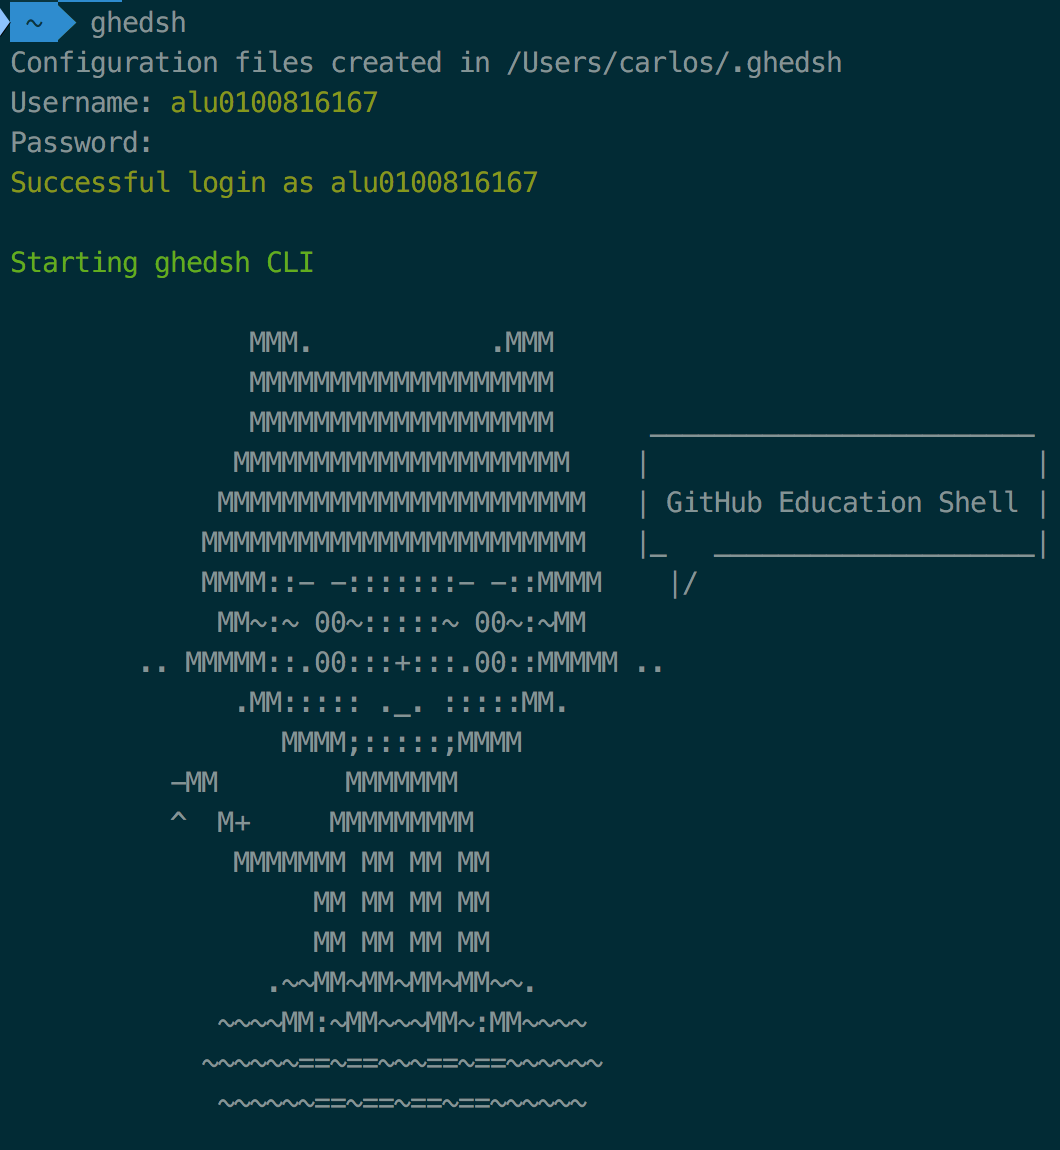
\includegraphics[width=0.68\textwidth]{images/login-example}
	\caption{Ejemplo de autenticación al usar ghedsh por primera vez.}
	\label{fig:masterv1}
	\end{center}
\end{figure}

%------------------------------------------------------------------------------------------------------------
\section{Comandos del núcleo de ghedsh}
\label{3:sec:2}

Como se ha indicado en la introducción de este tercer capítulo, se han separado, por un lado, los comandos del núcleo de {\it ghedsh} y, por otro, los comandos característicos de {\it ghedsh}.
\bigskip

En esta sección, se explicará este primer grupo de comandos, encargado de tareas relacionadas con el sistema operativo y, lo más importante, hacer que la herramienta sea agradable de manejar para el usuario. Además, se revisarán aspectos importantes de su implementación.

\subsection{bash (comando ghedsh)}
\label{3.2.1}

Permite interpretar un comando en la terminal del sistema operativo, sin salir de {\it ghedsh}.
\bigskip

\textbf{Sintaxis:} \verb bash  \verb <comando_terminal>  .
En la figura \ref{fig:bash-example}, se muestra un ejemplo de uso.
\begin{figure}[H]
	\begin{center}
	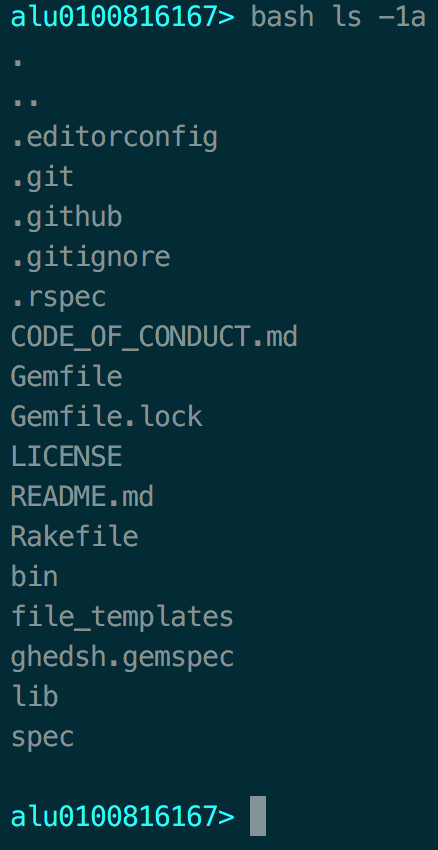
\includegraphics[width=0.30\textwidth]{images/bash-example}
	\caption{Ejemplo de uso del comando bash.}
	\label{fig:bash-example}
	\end{center}
\end{figure}

\subsection{Change directory: cd}
\label{3.2.2}
Análogamente al comando {\it cd} de la {\it Bash}\cite{B17}, que permite cambiar nuestro directorio actual de trabajo, en {\it ghedsh} también existe este comando. No obstante, aunque la idea es similar, existen diferencias a la hora de usarlo.
\bigskip

En nuestro sistema operativo (tipo Unix)\cite{B18}, cuando realizamos la operación {\it cd}, sólo podemos movernos entre directorios (dependiendo de los permisos). Dado que en {\it ghedsh} no existen directorios como tal, hablaremos de contextos.
Los contextos en esta herramienta hacen referencia a nivel de usuario, nivel de organización, nivel de repositorio, etcétera.
\bigskip

Imaginemos por un momento que nuestro usuario se llama \verb ejemplo , disponemos de un repositorio que se llama \verb ejemplo  y una organización denominada \verb ejemplo . Ésto es totalmente válido, puesto que lo que no permite GitHub es que dos usuarios se llamen igual, que el usuario tenga dos repositorios con el mismo nombre o dos organizaciones bajo el mismo nombre.
Entonces, debemos proporcionar alguna manera de desambiguar a qué contexto nos queremos cambiar.
\bigskip

En {\it ghedsh} se ha optado por el siguiente planteamiento: para realizar la operación de
{\it cd}, es necesario especificar el tipo de contexto (nivel) al que queremos cambiarnos, así, aunque el usuario se encuentre en el caso anteriormente comentado, {\it ghedsh} es capaz de saber a qué contexto debe cambiar.
La sintaxis del comando sería \verb cd  \verb <tipo>  \verb <nombre> , donde \verb nombre  es la cadena de texto que identifica al tipo.
\bigskip

Los tipos de contexto (pueden ser ampliables) que actualmente se soportan en {\it ghedsh} son:
\begin{itemize}
	\item \textbf{Nivel de usuario}: estando a nivel de usuario, éste se puede cambiar a cualquiera de sus repositorios o a cualquier organización a la que pertenezca, como vemos a continuación:
		\begin{itemize}
			\item Repositorio del usuario: \verb cd   \verb repo  \verb <nombre> .
			\item Organización del usuario: \verb cd   \verb org  \verb <nombre> . {\it ghedsh} soporta el autocompletado de organizaciones, es decir, se puede pulsar el tabulador para completar automáticamente el nombre de la organización.
		\end{itemize}
	\item \textbf{Nivel de organización}: estando a nivel de una organización de la que es miembro el usuario autenticado, ({\it ghedsh} sabrá que se refiere al entorno de la organización a la que se ha cambiado) se puede mover a:
		\begin{itemize}
			\item Repositorio de la organización: \verb cd   \verb repo  \verb <nombre> .
			\item Equipo de la organización: \verb cd   \verb team  \verb <nombre> .
		\end{itemize}
\end{itemize}

Además, si deseamos volver al contexto anterior, haremos de la misma manera que en sistemas operativos tipo Unix: \verb cd  \verb ..  . Hay que tener en cuenta que, actualmete, no se puede realizar la operación de volver al contexto anterior y cambiar a otro de manera simultánea (como en Unix \verb cd  \verb ../another/dir  ), es necesario hacerlo por separado.

\subsubsection{Detalles de implementación}
Puesto que se trata de uno de los comandos más importantes de {\it ghedsh}, se comentarán los aspectos destacados de la implementación del mismo, incluyendo las dificultades encontradas.
\bigskip

Internamente, el comando {\it cd} contiene una pila (stack\cite{B19}) en la que se almacenan todos los contextos previos. La estructura de un contexto se muestra en el siguiente fragmento de código:

\begin{lstlisting}[language=Ruby]
  config = {
    'User' => client.login.to_s,
  	'user_url' => client.web_endpoint.to_s << client.login.to_s,
    'Org' => nil,
    'org_url' => nil,
    'Repo' => nil,
    'repo_url' => nil,
    'Team' => nil,
    'team_url' => nil
  }
\end{lstlisting}

\begin{itemize}
	\item \verb User : permite saber el nombre del usuario autenticado en {\it ghedsh}.
	\item \verb user_url : contiene la URL ({\it Uniform Resource Locator}\cite{B20}) del perfil del usuairo en GitHub.
	\item \verb Org : indica el nombre de la organización actual, si el usuario no está posicionado sobre alguna, el valor es nulo.
	\item \verb org_url : URL de la organización en GitHub.
	\item \verb Repo : nombre del repositorio actual, en caso de estar dentro de alguno.
	\item \verb repo_url : URL del repositorio en GitHub.
	\item \verb Team : nombre del equipo actual si el usuario está posicionado dentro de alguno.
	\item \verb team_url : URL del equipo en GitHub.
\end{itemize}

En esencia, {\it change directory} irá variando estos parámetros para conocer a qué nivel se encuentra el usuario (\verb User  siempre tendrá un valor asignado porque representa el usuario autenticado).
Por ejemplo, para referirnos a un repositorio de una organización en la que el usuario es miembro, tendríamos:
\begin{lstlisting}[language=Ruby]
	config = {
    'User' => client.login.to_s,
  	'user_url' => client.web_endpoint.to_s << client.login.to_s,
    'Org' => "EXAMPLE-ORG",
    'org_url' => nil,
    'Repo' => "repository-within-example-org",
    'repo_url' => nil,
    'Team' => nil,
    'team_url' => nil
  }
\end{lstlisting}
En el caso de un repositorio de usuario, \verb User  tendría valor asignado y \verb Repo  también tendría valor asignado. A diferencia con el caso anterior, \verb Org  sería nulo ya que nos referimos a un repositorio a nivel de usuario.
\bigskip

Una de las dificultades en la implementación de este comando, fue que, antes de reasignar la estructura de datos que respresenta los contextos, era necesario almacenar el contexto actual para poder volver a éste más tarde.
\bigskip

Ruby proporciona dos métodos para copiar/clonar objetos: \verb dup \cite{B21} y \verb clone \cite{B22}. No obstante, realizan una copia superficial del objeto, es decir, crearán un nuevo identificador de objeto pero
el contenido del mismo referenciará al de la entidad original.
\bigskip

Para solucionarlo, se utilizó el módulo {\it Marshal}\cite{B23} de Ruby, que sí realiza una copia profunda del objeto.



%------------------------------------------------------------------------------------------------------------
\section{Comandos incorporados en ghedsh}
\label{3:sec:3}

A lo largo de esta sección, se explicarán individualmente los comandos característicos de {\it ghedsh}. Los comandos característicos o incorporados por {\it ghedsh}
son aquellos que trabajan con los datos de GitHub del usuario de la herramienta. Colaboran estrechamente con la GitHub API REST v3 (véase, para más detalle, la documentación oficial de {\it Octokit}\cite{B24}).
Se explicará la sintaxis para cada uno de ellos y se proporcionará ejemplos de uso.
\bigskip

Como convenio, los parámetros con el formato \verb <parameter> , son obligatorios. Los que tengan el formato \verb [parameter] , son opcionales.
\bigskip

Por otro lado, las expresiones regulares admiten las opciones establecidas por Ruby.

\subsection{clear}
\label{3.3.1}

Realiza la misma tarea que el comando \verb clear  en Bash. Borra la pantalla si es posible y sitúa el cursor en la parte superior izquierda de la pantalla (ignora cualquier parámetro adicional).

\textbf{Sintaxis}: \verb clear  .

\subsection{clone}
\label{3.3.2}

Clona repositorios y, si ya existe en el directorio local, realizará \verb git  \verb pull  \verb --all . Recibe como parámetro obligatorio el nombre del repositorio que se desea clonar o una expresión regular, que permitirá clonar todos los repositorios que casen con ella.
Opcionalmente, es posible especificar un directorio dentro de \verb $HOME   de la máquina local. En caso de no exisir, se creará. Por defecto, se clonarán en el directorio actual de la máquina local.

\textbf{Sintaxis}: \verb clone  \verb <nombre_repo|/Regexp/>  \verb [ruta_en_home]  .

Se puede ejecutar en:
\begin{itemize}
	\item Contexto de \textbf{usuario}: clonará los repositorios del usuario autenticado en {\it ghedsh}.
	\item Contexto de \textbf{organización}: clonará los repositorios de la organización en la que se encuentre posicionado.
\end{itemize}

En la figura \ref{fig:clone-example} y \ref{fig:clone-example-org} se muestran ejemplos de uso.

\begin{figure}[H]
	\begin{center}
	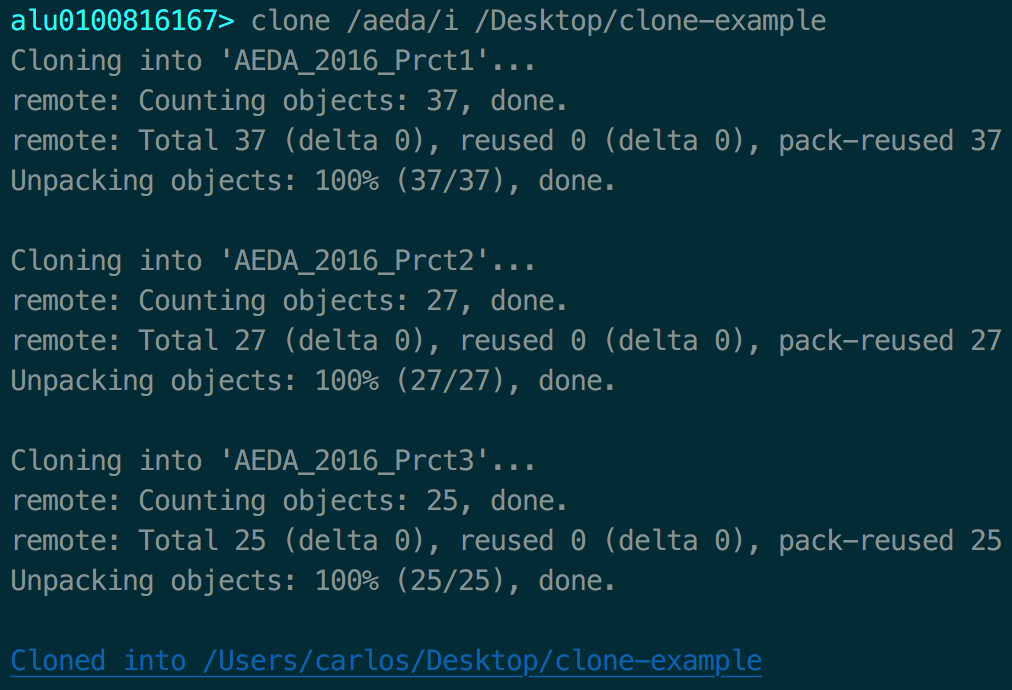
\includegraphics[width=0.60\textwidth]{images/clone-example}
	\caption{Ejemplo de clonar un repositorio de usuario.}
	\label{fig:clone-example}
	\end{center}
\end{figure}

\begin{figure}[H]
	\begin{center}
	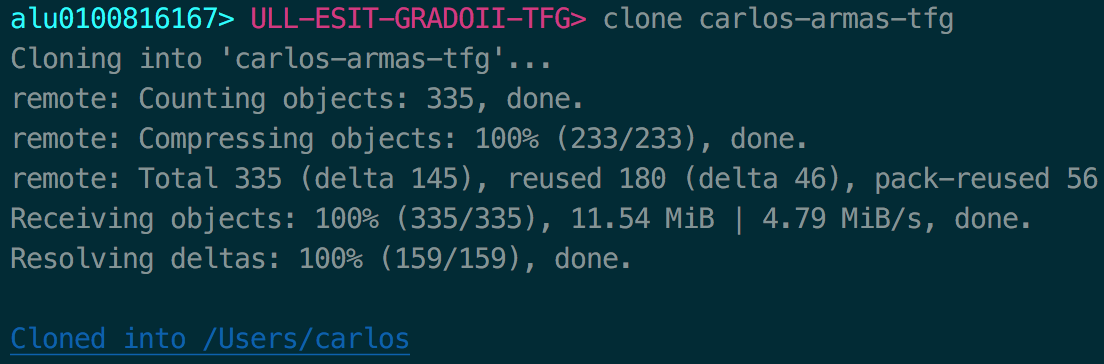
\includegraphics[width=0.60\textwidth]{images/clone-example-org}
	\caption{Ejemplo de clonar un repositorio de organización.}
	\label{fig:clone-example-org}
	\end{center}
\end{figure}

\subsection{commits}
\label{3.3.3}

Muestra los {\it commits} (SHA, fecha, autor y mensaje del {\it commit}) de la rama \verb master , en caso de que no se le pase como parámetro una rama en concreto.
Es necesario estar posicionado sobre un repositorio de cualquiera de los siguientes contextos: \textbf{organización} o \textbf{usuario}.

\textbf{Sintaxis}: \verb commits  \verb [rama_repositorio]  .

\begin{figure}[H]
	\begin{center}
	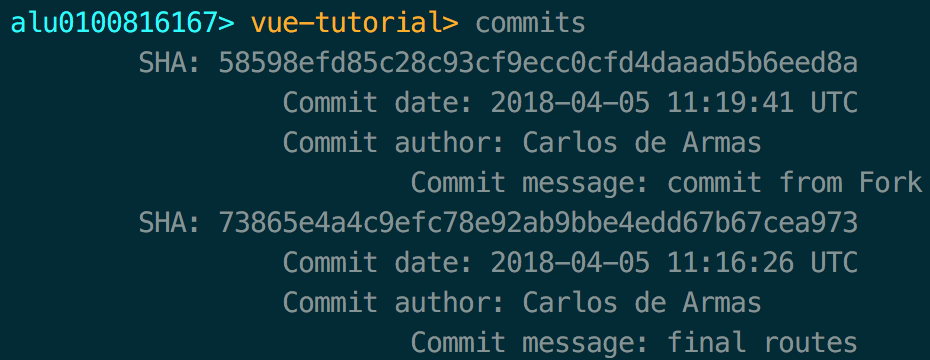
\includegraphics[width=0.59\textwidth]{images/user-commits}
	\caption{Mostrar commits en un repositorio de usuario.}
	\label{fig:user-commits}
	\end{center}
\end{figure}

\begin{figure}[H]
	\begin{center}
	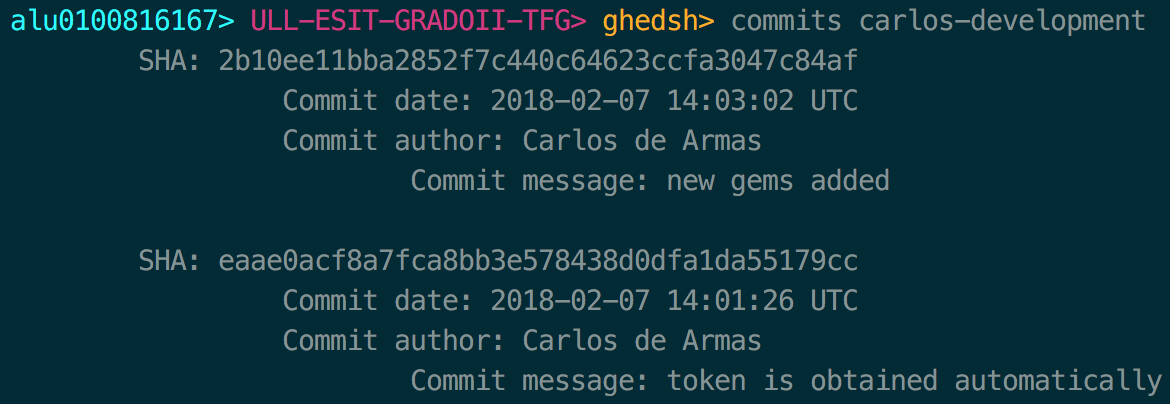
\includegraphics[width=0.59\textwidth]{images/orgs-commits}
	\caption{Mostrar commits de la rama de un repositorio de organización.}
	\label{fig:user-commits}
	\end{center}
\end{figure}

\subsection{exit}
\label{3.3.4}

Temina la ejecución de {\it ghedsh}, guardando el contexto actual. Es decir, si el usuario se encontraba dentro de una organización, la próxima vez que entre en {\it ghedsh} estará dentro de la organización.

\textbf{Sintaxis}: \verb exit  .

\subsection{files}
\label{3.3.5}

Muestra el contenido y el tipo de contenido  (fichero o directorio) de un repositorio. Debe estar posicionado dentro de un repositorio de \textbf{usuario} o repositorio de \textbf{organización}.
Si no se le proporciona ningún parámetro, muestra el contenido de la raíz del repositorio. Si se le especifica un subdirectorio, se mostrará su contenido.

\textbf{Sintaxis}: \verb files  \verb [subdirectorio]  . 

\begin{figure}[H]
	\begin{center}
	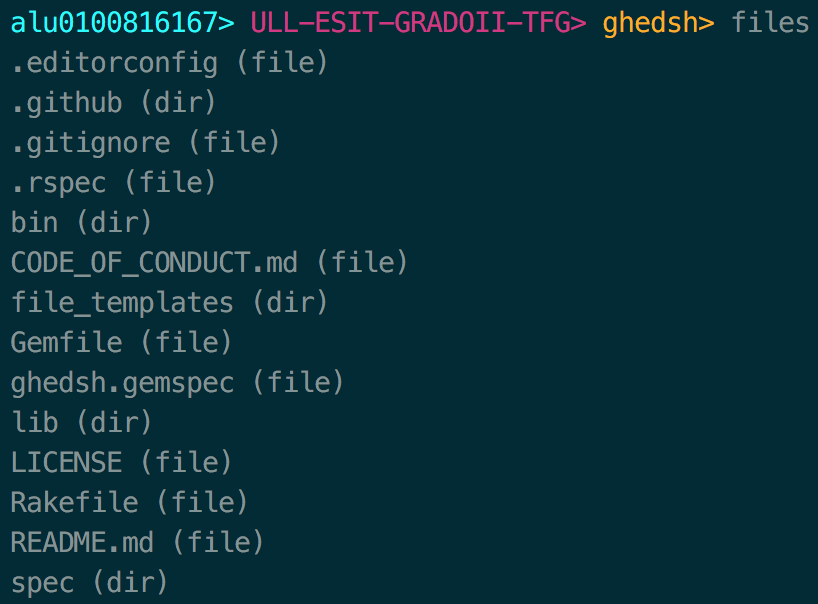
\includegraphics[width=0.5\textwidth]{images/dir-content}
	\caption{Listar contenido del repositorio.}
	\label{fig:dir-content}
	\end{center}
\end{figure}

\begin{figure}[H]
	\begin{center}
	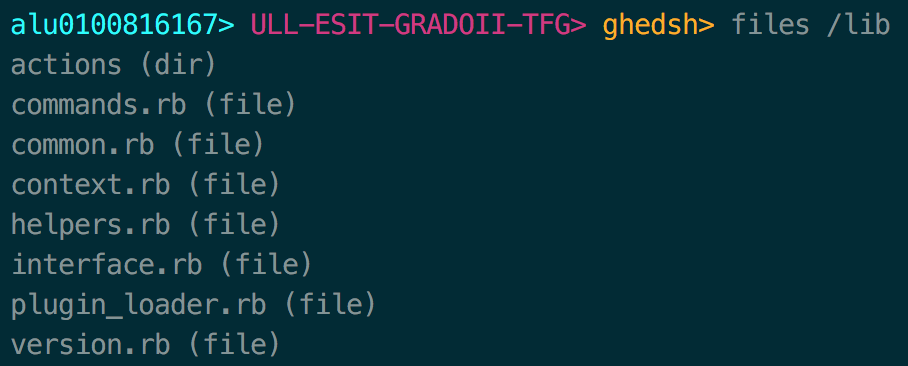
\includegraphics[width=0.5\textwidth]{images/subdir-content}
	\caption{Listar contenido de un subdirectorio.}
	\label{fig:subdir-content}
	\end{center}
\end{figure}

\subsection{invite\_member}
\label{3.3.6}

Añade nuevos miembros a una organización. Recibe como parámetros el/los nombres de usuario de GitHub, separados por comas o por espacios.

Sólo puede ejecutarse en el contexto de una \textbf{organización}.

\textbf{Sintaxis}: \verb invite_member  \verb <user1,  \verb user2,  \verb user3,  \verb ...,  \verb n>  .
 
\begin{figure}[H]
	\begin{center}
	
\includegraphics[width=1\textwidth]{images/invite-member}
	\caption{Añadir miembros específicos.}
	\label{fig:invite-member}
	\end{center}
\end{figure}

\subsection{invite\_member\_from\_file}
\label{3.3.7}

Añade  nuevos miembros a una organización, especificando su nombre de usuario en GitHub. Recibe como único parámetro un fichero (ver plantilla \cite{B27}) existente en \verb $HOME  de la máquina local. 

El comando se ejecuta, exclusivamente, dentro del contexto de una \textbf{organización}.

\textbf{Sintaxis}: \verb invite_member_from_file  \verb <ruta_home_fichero>  .

\begin{figure}[H]
	\begin{center}
	
\includegraphics[width=1\textwidth]{images/add-members-file}
	\caption{Añadir miembros mediante fichero.}
	\label{fig:add-members-fil}
	\end{center}
\end{figure}

\subsection{invite\_outside\_collaborators}
\label{3.3.8}

Invita a ser miembros de la organización a los colaboradores externos de la misma. Si no se especifica ningún parámetro, invita a todos los colaboradores externos. En caso de que reciba un parámetro, tendrá que ser un fichero (ver plantilla \cite{B26}) situado en \verb $HOME  de la máquina local.

Se ejecuta, exclusivamente, cuando el usuario de {\it ghedsh} está situado en el contexto de una \textbf{organización}.

\textbf{Sintaxis}: \verb invite_outside_collaborators  \verb [ruta_home_fichero]  .

\begin{figure}[H]
	\begin{center}
	
\includegraphics[width=1\textwidth]{images/invite-collabs}
	\caption{Invitación a ser miembros desde fichero.}
	\label{fig:invite-collabs}
	\end{center}
\end{figure}

\subsection{issues}
\label{3.3.9}
Abre el navegador por defecto, situando al usuario en la lista de incidencias ({\it issues}). Debe estar posicionado dentro de un repositorio de \textbf{usuario} o repositorio de \textbf{organización}.

\textbf{Sintaxis}: \verb issues  .

\begin{figure}[H]
	\begin{center}
	
\includegraphics[width=0.65\textwidth]{images/list-issues}
	\caption{Ver incidencias de un repositorio.}
	\label{fig:list-issues}
	\end{center}
\end{figure}

\begin{figure}[H]
	\begin{center}
	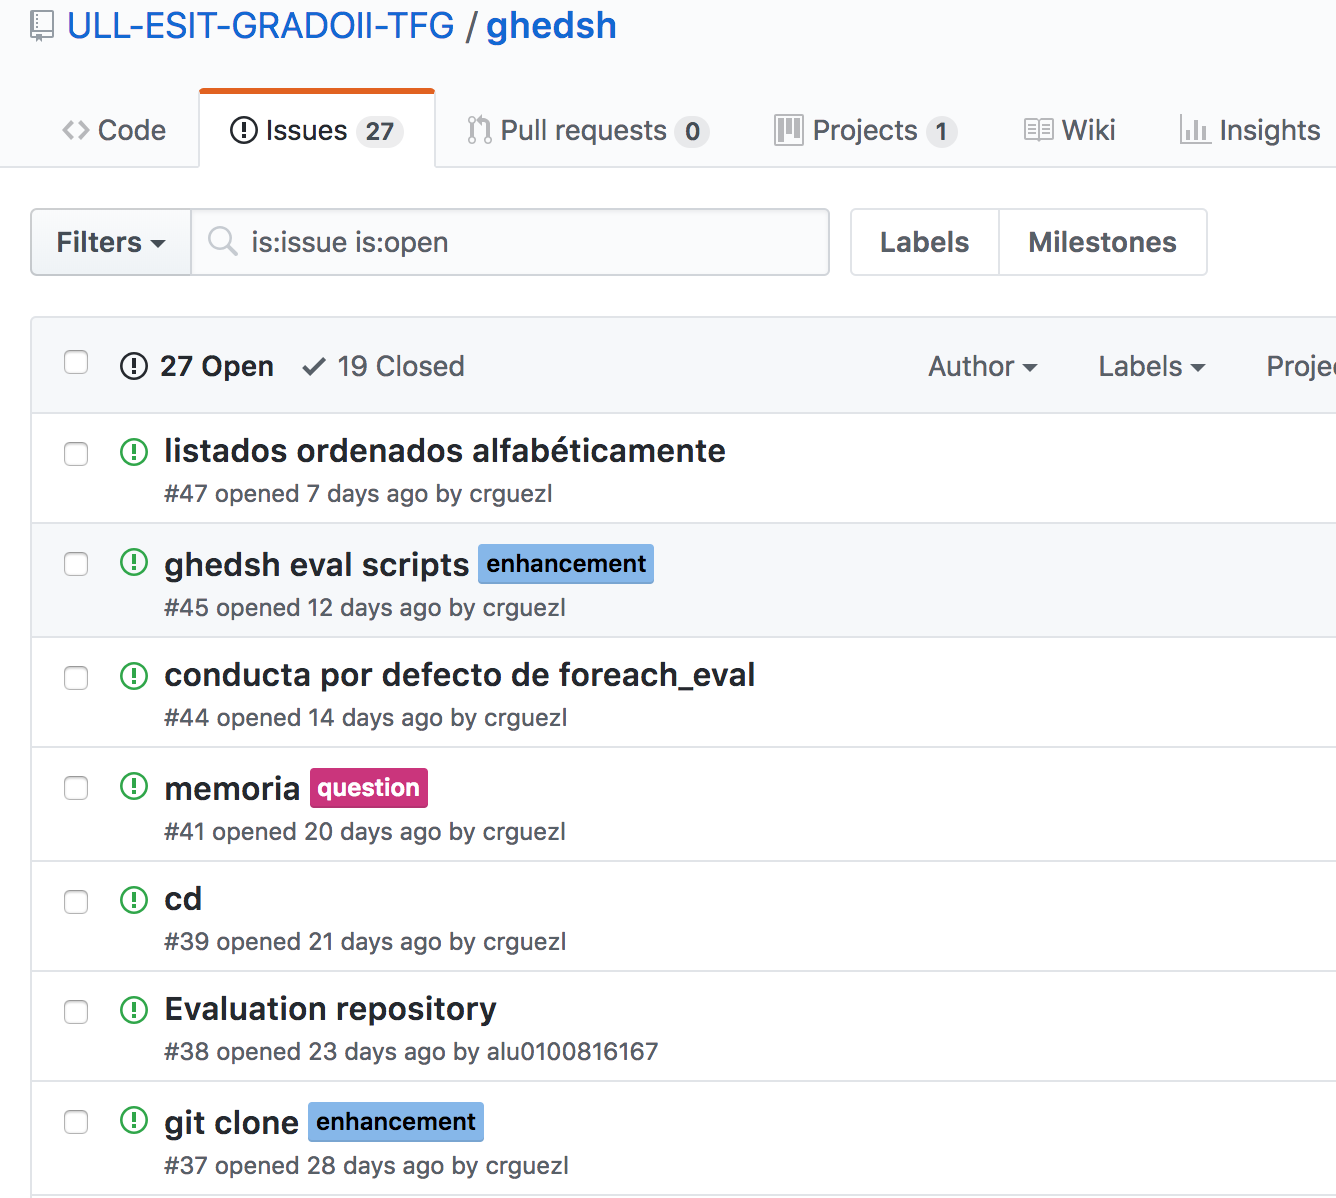
\includegraphics[width=0.65\textwidth]{images/issues-list}
	\caption{Listado de incidencias del repositorio en GitHub.}
	\label{fig:issues-list}
	\end{center}
\end{figure}

\subsection{new\_issue}
\label{3.3.10}

Abre el navegador por defecto, situando al usuario en el formulario de creación de un issue. Para ejecutarlo, es necesario estar posicionado sobre un repositorio.

\textbf{Sintaxis}: \verb new_issue  .

Está disponible para:
\begin{itemize}
	\item Contexto \textbf{usuario}: abre la página de {\it issues} del repositorio de usuario en el que está posicionado.
	\item Contexto \textbf{organización}: abre la página de {\it issues} del repositorio de la organización sobre la que está posicionado.
\end{itemize}
\begin{figure}[H]
	\begin{center}
	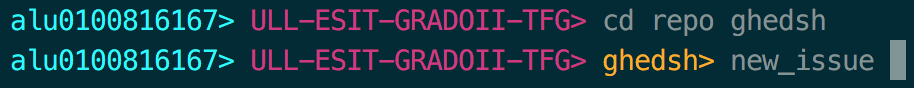
\includegraphics[width=0.7\textwidth]{images/new-issue}
	\caption{Nuevo issue en repositorio de organización.}
	\label{fig:new-issue}
	\end{center}
\end{figure}

\begin{figure}[H]
	\begin{center}
	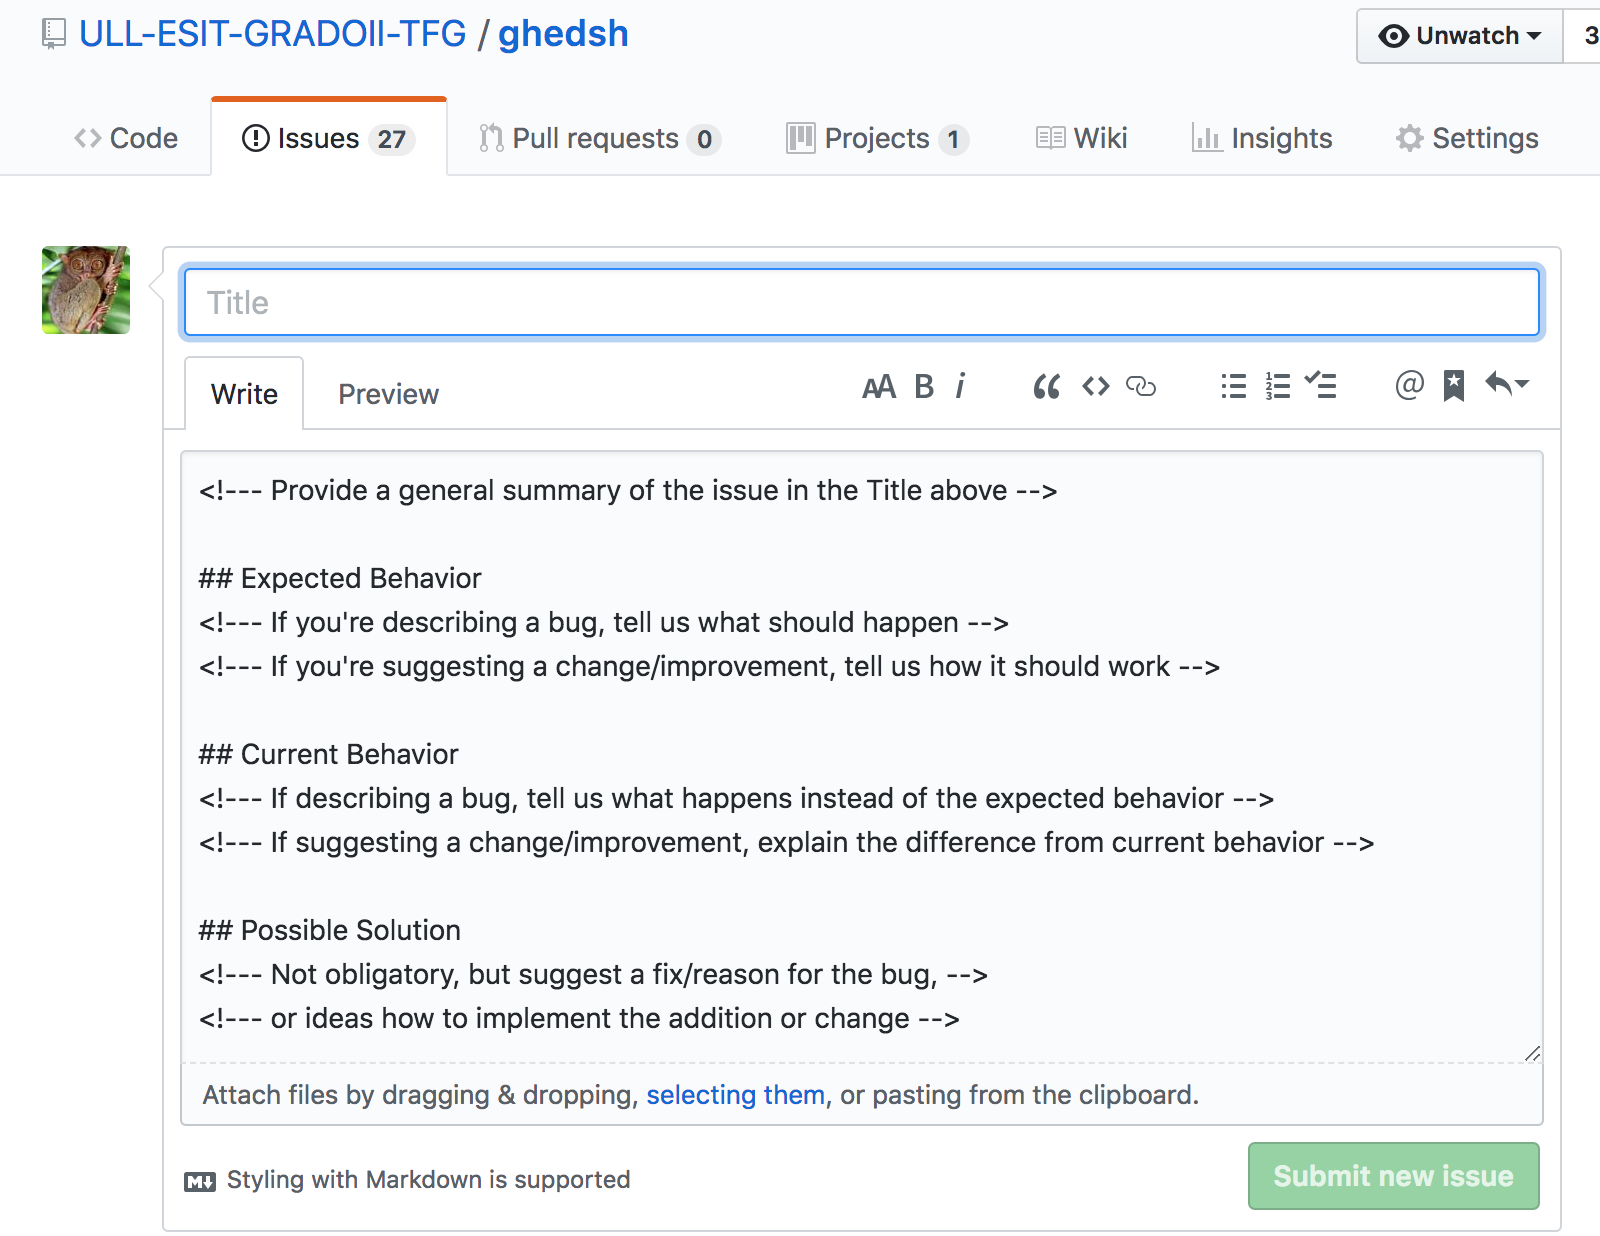
\includegraphics[width=0.7\textwidth]{images/issue-form}
	\caption{Formulario de creación de incidencias (issues).}
	\label{fig:new-issue}
	\end{center}
\end{figure}

\subsection{new\_repo}
\label{3.3.11}

Crea un nuevo repositorio. La herramienta muestra al usuario dos opciones para crearlo (menú):
\begin{itemize}
	\item {\it Default}: crea un repositorio público.
	\item {\it Custom}: crea un repositorio público o privado, al que es posible añadirle opciones específicas mediante una guía que se le mostrará.
	Si no se quiere especificar alguna de las opciones que se muestran, puede pulsar la tecla retorno y omitir el paso.
\end{itemize}
\textbf{Sintaxis}: \verb new_repo  \verb <nombre_repositorio> .
Disponible para:
\begin{itemize}
	\item Contexto \textbf{usuario}: crea un repositorio para el usuario autenticado.
	\item Contexto \textbf{organización}: crea un repositorio dentro de la organización en la que se encuentre posicionado el usuario.
\end{itemize}
En la figura \ref{fig:create-repo}, vemos el menú de creación del repositorio.
\begin{figure}[H]
	\begin{center}
	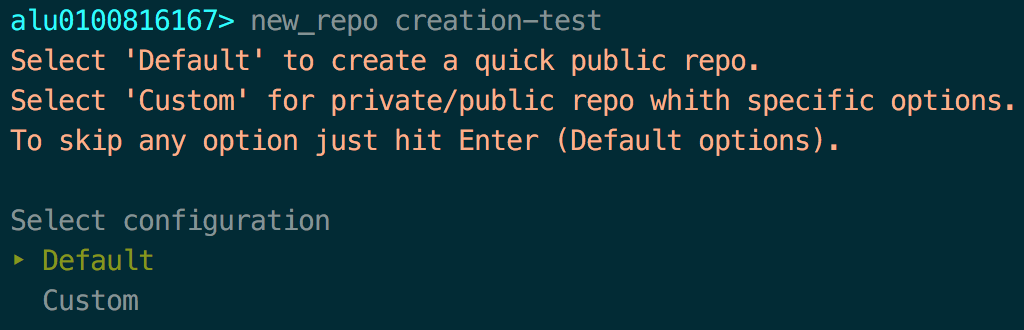
\includegraphics[width=0.70\textwidth]{images/create-repo}
	\caption{Menú para la creación de un repositorio.}
	\label{fig:create-repo}
	\end{center}
\end{figure}

\begin{figure}[H]
	\begin{center}
	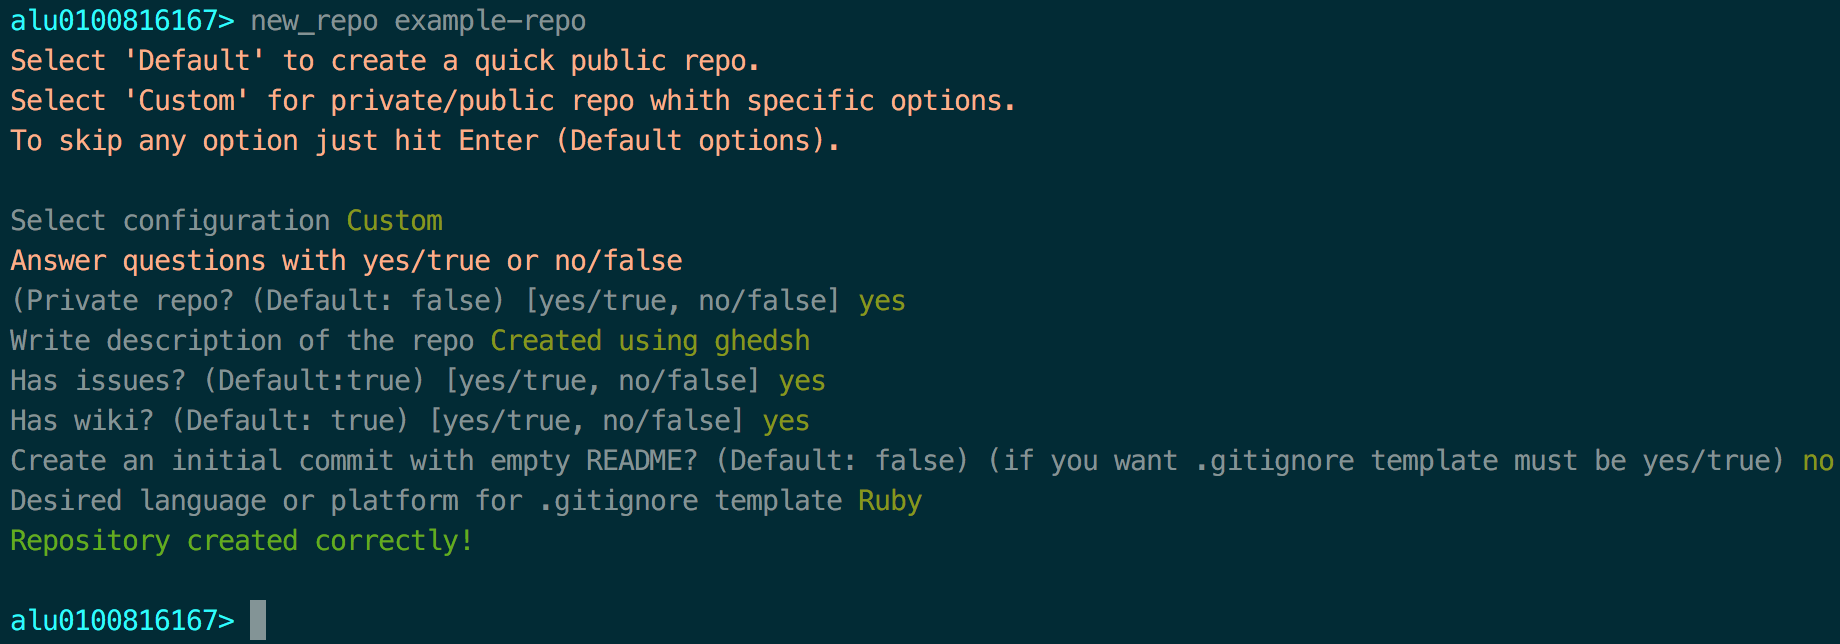
\includegraphics[width=1\textwidth]{images/custom-repo}
	\caption{Creación de un repositorio de usuario con opciones específicas.}
	\label{fig:custom-repo}
	\end{center}
\end{figure}

\subsection{new\_team}
\label{3.3.12}

Crea un nuevo equipo dentro de la organización en la que esté posicionado el usuario. Si el comando no recibe ningún parámetro, se abrirá la URL del formulario para crear el equipo en la web de GitHub. En caso de especificarle un parámetro,
éste tiene que ser un fichero (ver plantilla \cite{B25}) que se encuentre en algún lugar de \verb $HOME  en la máquina local.

Una vez más, este comando sólo se puede ejecutar cuando el usuario está posicionado dentro de una organización en {\it ghedsh}.

\textbf{Sintaxis}: \verb new_team  \verb [ruta_home_fichero]  .

\begin{figure}[H]
	\begin{center}
	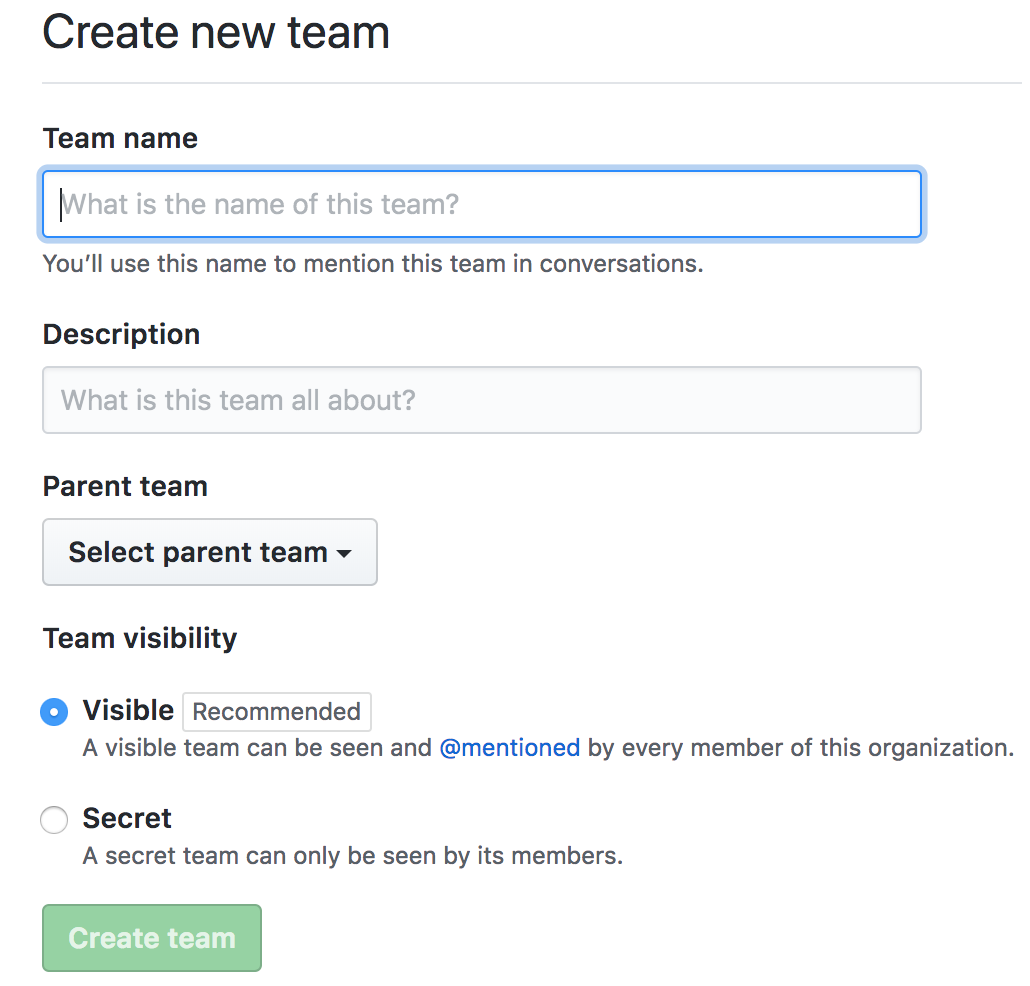
\includegraphics[width=0.59\textwidth]{images/create-team-form}
	\caption{Formulario de creación de un equipo en GitHub.}
	\label{fig:create-team-form}
	\end{center}
\end{figure}

\begin{figure}[H]
	\begin{center}
	
\includegraphics[width=0.9\textwidth]{images/create-team-file}
	\caption{Creación de un equipo mediante fichero.}
	\label{fig:create-team-file}
	\end{center}
\end{figure}

\subsection{open}
\label{3.3.13}

Abre el navegador por defecto y muestra información de GitHub según el contexto:
\begin{itemize}
	\item Contexto de \textbf{usuario}: si se ejecuta \verb open  a nivel de usuario, se abre en el navegador el perfil GitHub del usuario autenticado en {\it ghedsh}. En caso de estar en un repositorio de usuario, se abre la URL de este repositorio.
	\item Contexto de \textbf{organización}: a nivel de organización abre el perfil de la organización en GitHub. Si el usuario se encuentra posicionado en un repositorio de la organización, abre la URL del repositorio.
	Para este contexto en concreto, es posible pasarle un parámetro que consista en una expresión regular o el nombre de algún miembro y abrir su perfil.
	En este caso, la \textbf{sintaxis} sería: \verb open  \verb "nombre"  (para el nombre del miembro) o bien \verb open  \verb /Regexp/  .
	\item Contexto de \textbf{equipo}: abre la URL del equipo en GitHub.
\end{itemize}

\textbf{Sintaxis} general: \verb open  .

\subsection{orgs}
\label{3.3.14}

Muestra las organizaciones a las que pertenece el usuario autenticado en {\it ghedsh}. Si el comando no recibe ningún parámetro, se mostrarán todas las organizaciones. En caso de proporcionarle un parámetro, debe ser una expresión regular y mostrará los resultados que casen.

Sólo está disponible en contexto de \textbf{usuario}.

\textbf{Sintaxis}: \verb orgs  \verb [/Regexp/]  .

\begin{figure}[H]
	\begin{center}
	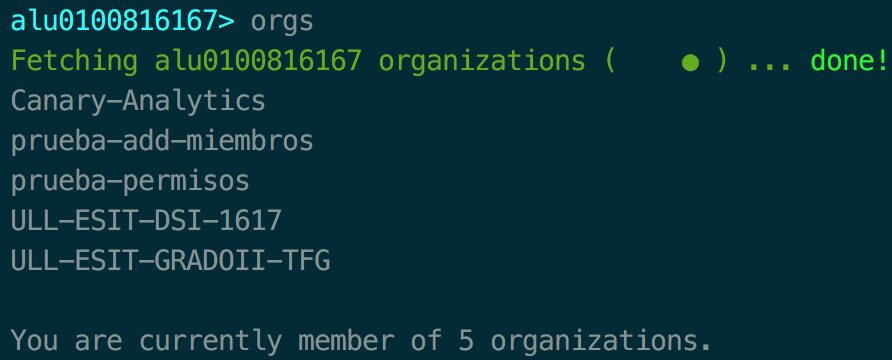
\includegraphics[width=0.59\textwidth]{images/show-all-orgs}
	\caption{Mostrar todas las organizaciones del usuario autenticado en ghedsh.}
	\label{fig:show-orgs-regexp}
	\end{center}
\end{figure}

\begin{figure}[H]
	\begin{center}
	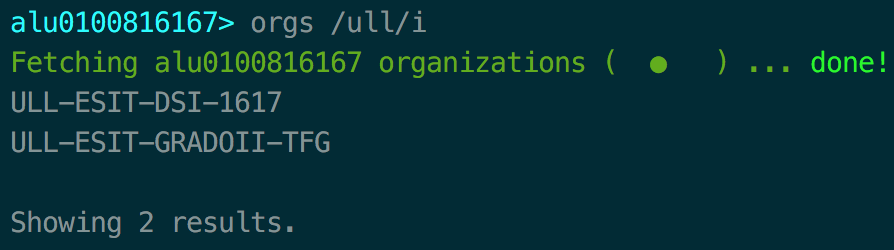
\includegraphics[width=0.59\textwidth]{images/show-orgs-regexp}
	\caption{Filtrar organizaciones mediante expresión regular.}
	\label{fig:show-orgs-regexp}
	\end{center}
\end{figure}

\subsection{people}
\label{3.3.15}

Muestra los nombres de los usuarios que componen una organización. Esto incluye miembros y colaboradores externos (si el usuario autenticado en {\it ghedsh} tiene permisos de administrador en la organización).
Si no se le proporciona ningún parámetro, lista todos. En caso de utilizar una expresión regular, se mostrarán los resultados que hayan casado con ella.

Este comando se usa, exclusivamente, cuando el usuario está posicionado dentro del contexto de una \textbf{organización}.

\textbf{Sintaxis}: \verb people  \verb [/Regexp/]  .

\begin{figure}[H]
	\begin{center}
	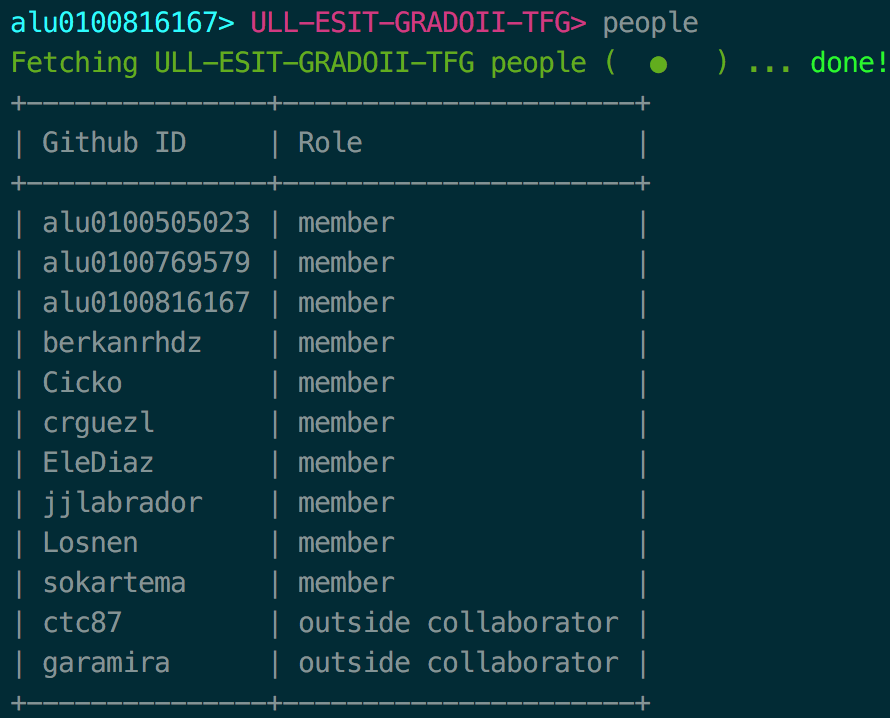
\includegraphics[width=0.59\textwidth]{images/org-people}
	\caption{Mostrar los miembros de una organización.}
	\label{fig:org-people}
	\end{center}
\end{figure}

\begin{figure}[H]
	\begin{center}
	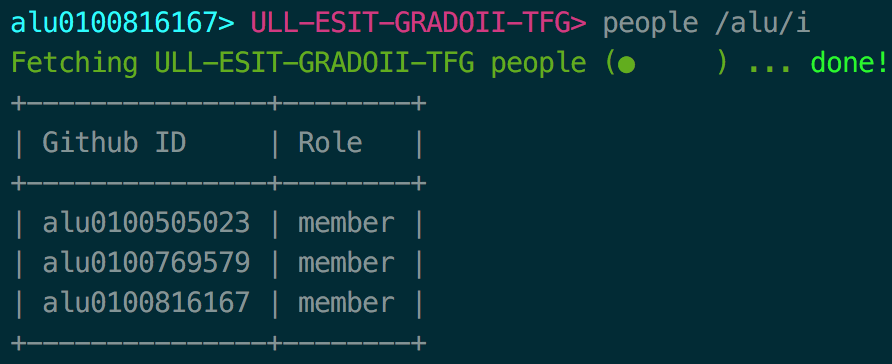
\includegraphics[width=0.59\textwidth]{images/org-people-regexp}
	\caption{Mostrar mediante expresión regular los miembros de una organización.}
	\label{fig:org-people-regexp}
	\end{center}
\end{figure}

\subsection{repos}
\label{3.3.16}

Muestra los repositorios según el contexto. Si no se le especifica nungún parámetro, mostrará todos los repositorios. Si se le proporciona una expresión regular, mostrará los nombres de los repositorios que hayan casado.

\textbf{Sintaxis}: \verb repos \verb [/Regexp/] .
\begin{itemize}
	\item Contexto \textbf{organización}: muestra los repositorios de la organización en la que se encuentra el usuario de {\it ghedsh}.
	\begin{figure}[H]
		\begin{center}
		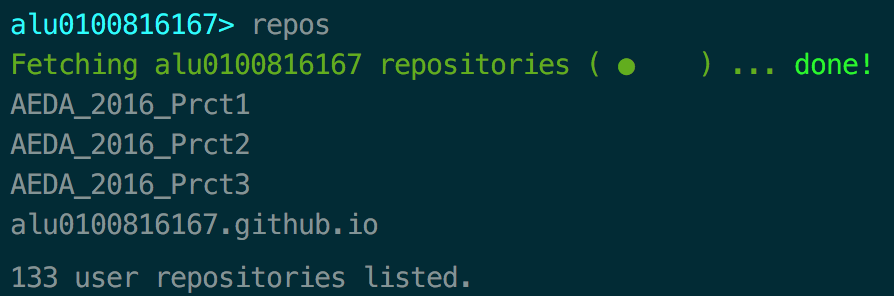
\includegraphics[width=0.60\textwidth]{images/user-repos}
		\caption{Comando repos a nivel de usuario.}
		\label{fig:user-repos}
		\end{center}
	\end{figure}
	\item Contexto \textbf{usuario}: muestra los repositorios del usuario autenticado en {\it ghedsh}.
	\begin{figure}[H]
		\begin{center}
		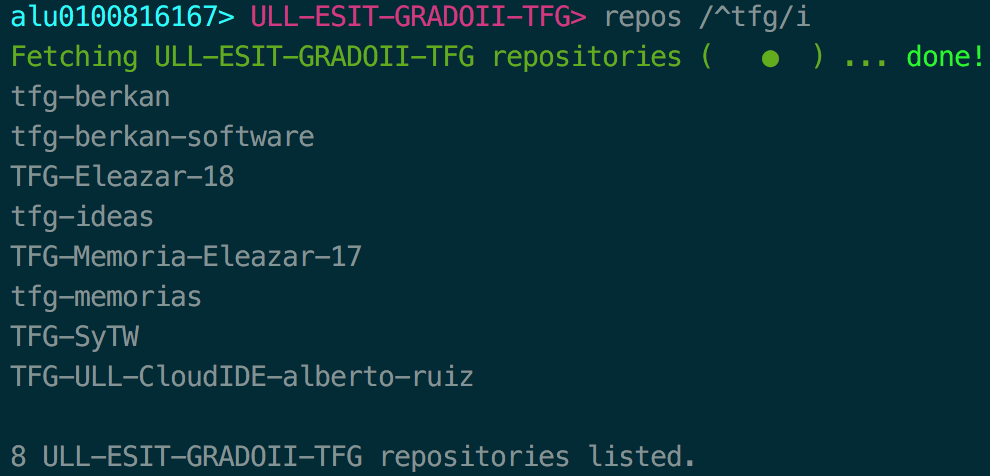
\includegraphics[width=0.70\textwidth]{images/org-repos}
		\caption{Comando repos a nivel de organización.}
		\label{fig:org-repos}
		\end{center}
	\end{figure}
\end{itemize}

\subsection{rm\_repo}
\label{3.3.17}

Elimina el repositorio especificado. Se puede realizar tanto a nivel de \textbf{usuario} como a nivel de \textbf{organización}.

\textbf{Sintaxis}: \verb rm_repo  \verb <nombre_repositorio>  .

\begin{figure}[H]
	\begin{center}
	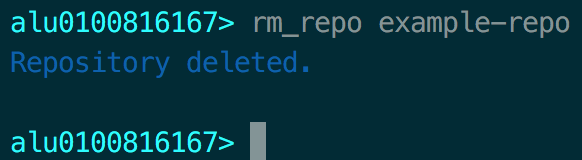
\includegraphics[width=0.5\textwidth]{images/delete-repo}
	\caption{Eliminación de un repositorio.}
	\label{fig:custom-repo}
	\end{center}
\end{figure}

\subsection{rm\_team}
\label{3.3.18}

Elimina un equipo. No recibe ningún parámetro. Se abre el navegador por defecto y el usuario borrará el o los equipos que desee de la lista proporcionada. Se ejecuta sólo en contexto de \textbf{organización}.

\textbf{Sintaxis}: \verb rm_team  .

\subsection{teams}
\label{3.3.19}

Muestra los equipos existentes en una organización. Si no se le especifica ningún parámetro, listará todos los equipos. Si se le proporciona una expresión regular, mostrará los resultados que casen con ella.
Se ejecuta, exclusivamente, en el contexto de una \textbf{organización}.

\textbf{Sintaxis}: \verb teams  \verb [/Regexp/]  .

\begin{figure}[H]
	\begin{center}
	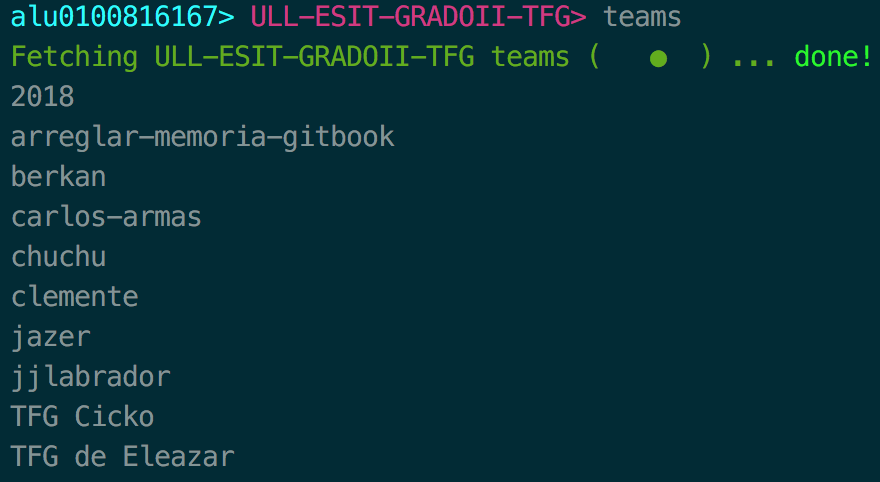
\includegraphics[width=0.59\textwidth]{images/org-teams}
	\caption{Listar los equipos de una organización.}
	\label{fig:org-teams}
	\end{center}
\end{figure}

\begin{figure}[H]
	\begin{center}
	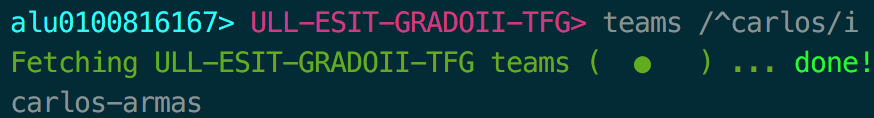
\includegraphics[width=0.59\textwidth]{images/org-regexp-teams}
	\caption{Listar mediante expresión regular los equipos de una organización.}
	\label{fig:org-regexp-teams}
	\end{center}
\end{figure}

%------------------------------------------------------------------------------------------------------------
\section{Comandos que dan soporte al proceso de evaluación}
\label{3:sec:4}

Los comandos que se explicarán en esta sección reflejan uno de los principales objetivos de {\it ghedsh}: aportar funcionalidades específicas
que usen las metodologías de {\it GitHub Education}, facilitando al profesorado la gestión de repositorios del alumnado así como la ejecución de {\it scripts} sobre los mismos.
\bigskip

En este conjunto de comandos tenemos: \verb new_eval , \verb foreach  y \verb foreach_try .

\subsection{new\_eval}
\label{3.4.1}

Permite crear un repositorio de evaluación. Recibe como parámetros el nombre del repositorio de evaluación y una expresión regular que añade como subdirectorios los repositorios que lo conforman. En {\it ghedsh}, un repositorio de evaluación consiste en hacer uso de los submódulos de {\it git}, de manera que se crea un repositorio raíz que contiene como submódulos
todos los proyectos que se van a evaluar. Los pasos que realiza son:
\begin{itemize}
	\item En el directorio actual de la máquina local del usuario, crea un directorio con el mismo nombre del repositorio de evaluación.
	\item Añade como submódulos los repositorios de la organización que casen con la expresión regular.
	\item Ejecuta \verb git  \verb push   y sube el contenido a la plataforma GitHub.
\end{itemize}
\bigskip

Dado que, para comprender todas las ventajas que ofrece este comando, es necesario conocer los submódulos de git ({\it gitsubmodules\cite{B28}}), se explicará en qué consisten a continuación.
\bigskip

Esencialmente, un submódulo es un repositorio que se encuentra contenido dentro de otro repositorio. El submódulo tiene su propio histórico de {\it commits} y, el repositorio raíz que lo contiene, se denomina súper-proyecto o súper-repositorio.
\bigskip

Es probable que, mientras trabajamos en un proyecto, necesitemos usar otro proyecto dentro de él. Quizás se trate de una librería de terceros o una que desarrollamos nosotros mismos de forma separada dentro de un proyecto principal. En estos casos, surge un problema común:
precisamos de ser capaces de tratar los dos proyectos por separado y, aún así, usar uno dentro del otro.
\bigskip

El control de versiones {\it Git} aborda ese problema usando submódulos. Los submódulos permiten mantener un repositorio como un subdirectorio de otro repositorio {\it Git}. Por lo tanto, permite clonar otro repositorio en nuestro proyecto, separando los {\it commits} de cada uno.
\bigskip

En {\it ghedsh}, el comando \verb new_eval  se encuentra disponible únicamente en el contexto de \textbf{organización}.

\textbf{Sintaxis}: \verb new_eval  \verb <nombre_repo_evaluacion>  \verb </Regexp/>  .

\begin{figure}[H]
	\begin{center}
	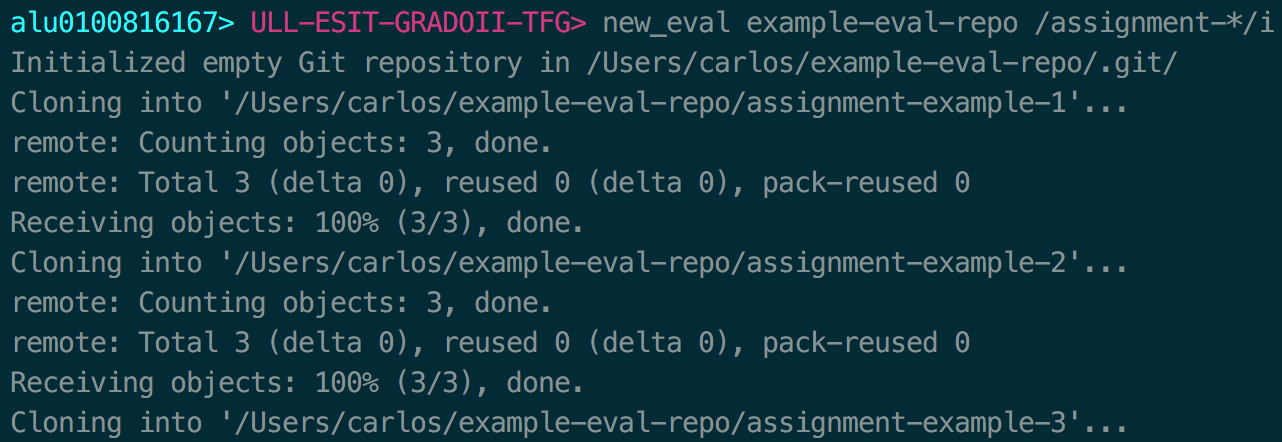
\includegraphics[width=0.9\textwidth]{images/eval-example}
	\caption{Ejemplo de creación de un repositorio de evaluación.}
	\label{fig:eval-example}
	\end{center}
\end{figure}

\begin{figure}[H]
	\begin{center}
	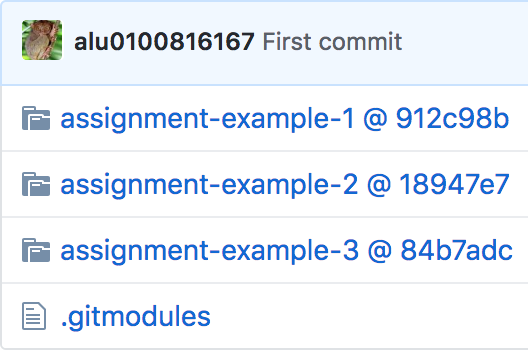
\includegraphics[width=0.4\textwidth]{images/eval-preview}
	\caption{Estructura de un repositorio de evaluación en GitHub.}
	\label{fig:eval-example}
	\end{center}
\end{figure}

\subsection{foreach}
\label{3.4.2}

Ejecuta sobre cada submódulo el comando {\it Bash} especificado como parámetro. No se detiene ante posibles errores en el proceso. Internamente, ejecuta \verb git  \verb submodule  \verb foreach  .

\textbf{Sintaxis}: \verb foreach  \verb <comando_bash>  .

Para que el comando lleve a cabo su cometido, se necesita lo siguiente:
\begin{itemize}
	\item Estar en contexto de \textbf{organización} dentro de {\it ghedsh} (único contexto en el que está disponible \verb foreach  ).
	\item Estar posicionado dentro de un repositorio que contenga submódulos, dentro de {\it ghedsh}.
	\item En la máquina local, el directorio actual (donde hemos ejecutado {\it ghedsh}) debe ser el repositorio de evaluación en cuestión.
\end{itemize}

Como se indica en la documentación oficial de  {\it git submodule foreach \cite{B29}}, el comando que se le proporciona tiene acceso a las siguientes variables:
\begin{itemize}
	\item \verb $name : nombre del submódulo.
	\item \verb $path : nombre del submódulo relativo al súper-proyecto.
	\item \verb $sha1 : SHA-1\cite{B30} del último {\it commit}.
	\item \verb $toplevel : ruta absoluta al súper-proyecto.
\end{itemize}

Por otro lado, como también indica la documentación, cuando existe un error en algún submódulo durante la ejecución del comando, se detiene y devuelve un código distinto de cero.
No obstante, este comportamiento puede evitarse añadiendo \verb ||  \verb :  al final del comando especificado como parámetro.
\bigskip

Hay que tener en cuenta que {\it foreach} en  \textbf{\it ghedsh}, \textbf{ya incorpora este comportamiento} y no se detendrá ante errores.

\begin{figure}[H]
	\begin{center}
	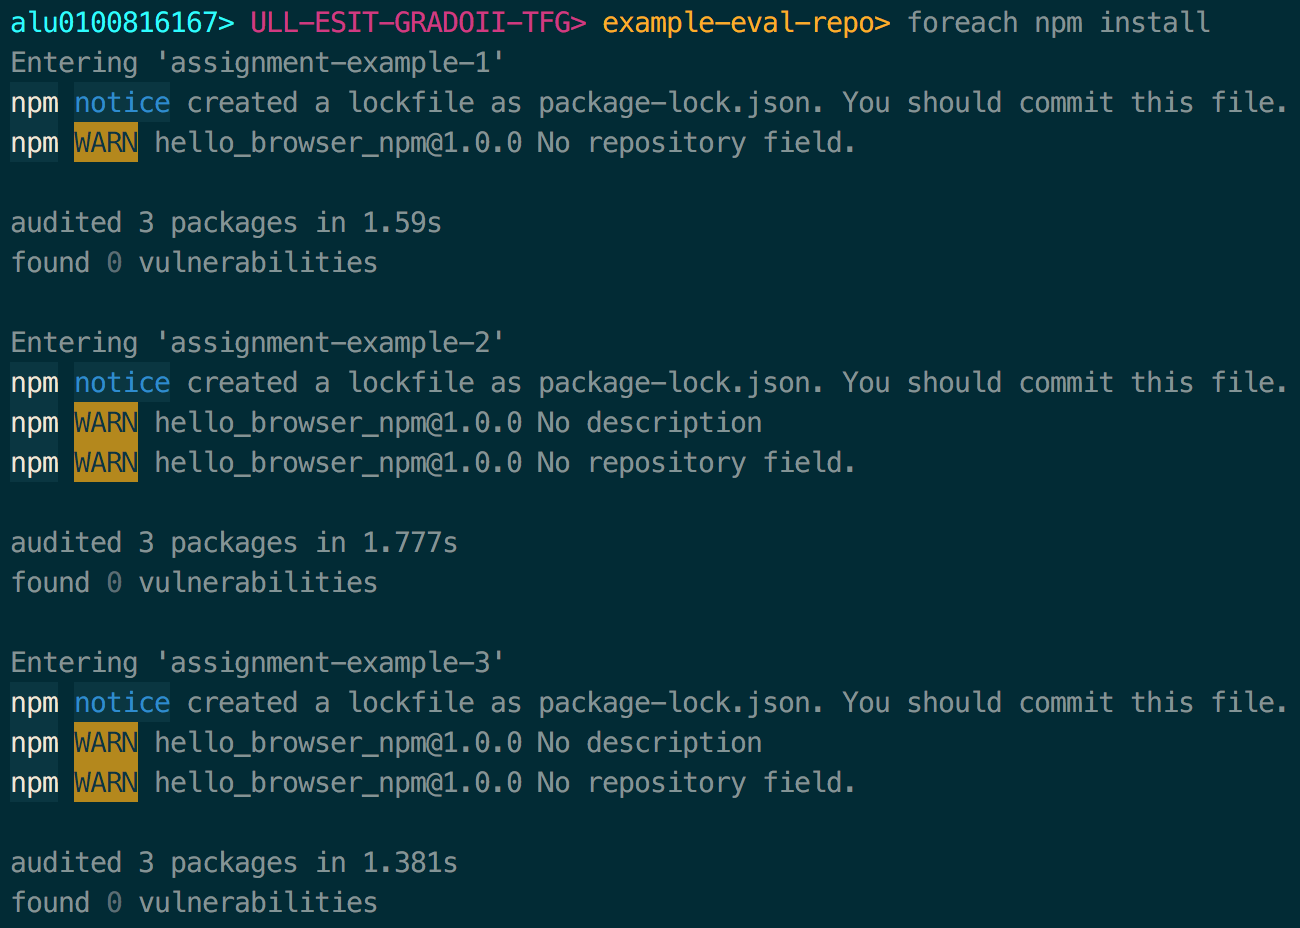
\includegraphics[width=0.9\textwidth]{images/foreach-example}
	\caption{Ejemplo de ghedsh foreach.}
	\label{fig:foreach-example}
	\end{center}
\end{figure}

\subsection{foreach\_try}
\label{3.4.3}

Realiza la misma tarea que {\it foreach}(\ref{3.4.2}) y requiere las mismas condiciones para su uso. A diferencia de éste, {\it foreach\_try} \textbf{detendrá su ejecución cuando se produzca un error en el proceso}.

\section{Caso de uso}
\label{3:sec:5}

Cabe destacar que el director de este Trabajo de Fin de Grado, Casiano Rodríguez León, ha hecho uso de la herramienta {\it ghedsh} en un entorno educativo real.
\bigskip

En concreto, se ha utilizado para facilitar tareas de gestión de repositorios y evaluación de prácticas en el curso de Procesadores de Lenguajes (año académico 2017-2018) a lo largo del mes de junio. Además, esto ha contribuido a mejorar aspectos de la herramienta,
puesto que, en un entorno real, suelen aparecer nuevos casos de uso que han sido cubiertos satisfactoriamente.
\bigskip

Por otro lado, Casiano ha realizado diversos vídeo tutoriales en los que se profundiza en el manejo de comandos que dan soporte al proceso de evaluación.


